\subsection{Basic Properties of Graphene}

Graphene is a two dimensional hexagonal atomic structure (also called honeycomb structure) made of carbon atoms. After its discovery in 2004\cite{novoselov}, graphene has sparked increasing interest among scientists due to its extraordinary mechanical\cite{strength}, optical\cite{optical} and electrical\cite{carrier} properties. This includes being a semiconductor without a band gap\cite{Lherbier2012}, high carrier mobility\cite{carrier} and an enormous intrinsic tensile strength\cite{strength}.

\subsubsection{Graphene Lattice}

Graphene is a two dimensional allotrope of carbon where atoms are densely packed in a hexagonal pattern with a distance of about \SI{1.42}{\angstrom} as shown in figure~\ref{fig:spm}. Each sp$^2$-hybridized carbon atom has a covalent $\sigma$-bond to three other carbon atoms formed from three of the valence electrons while the 4th valence electron does not participate in the covalent bonding but forms a conduction $\pi$-band.

\begin{figure}[!h]
  \centering
  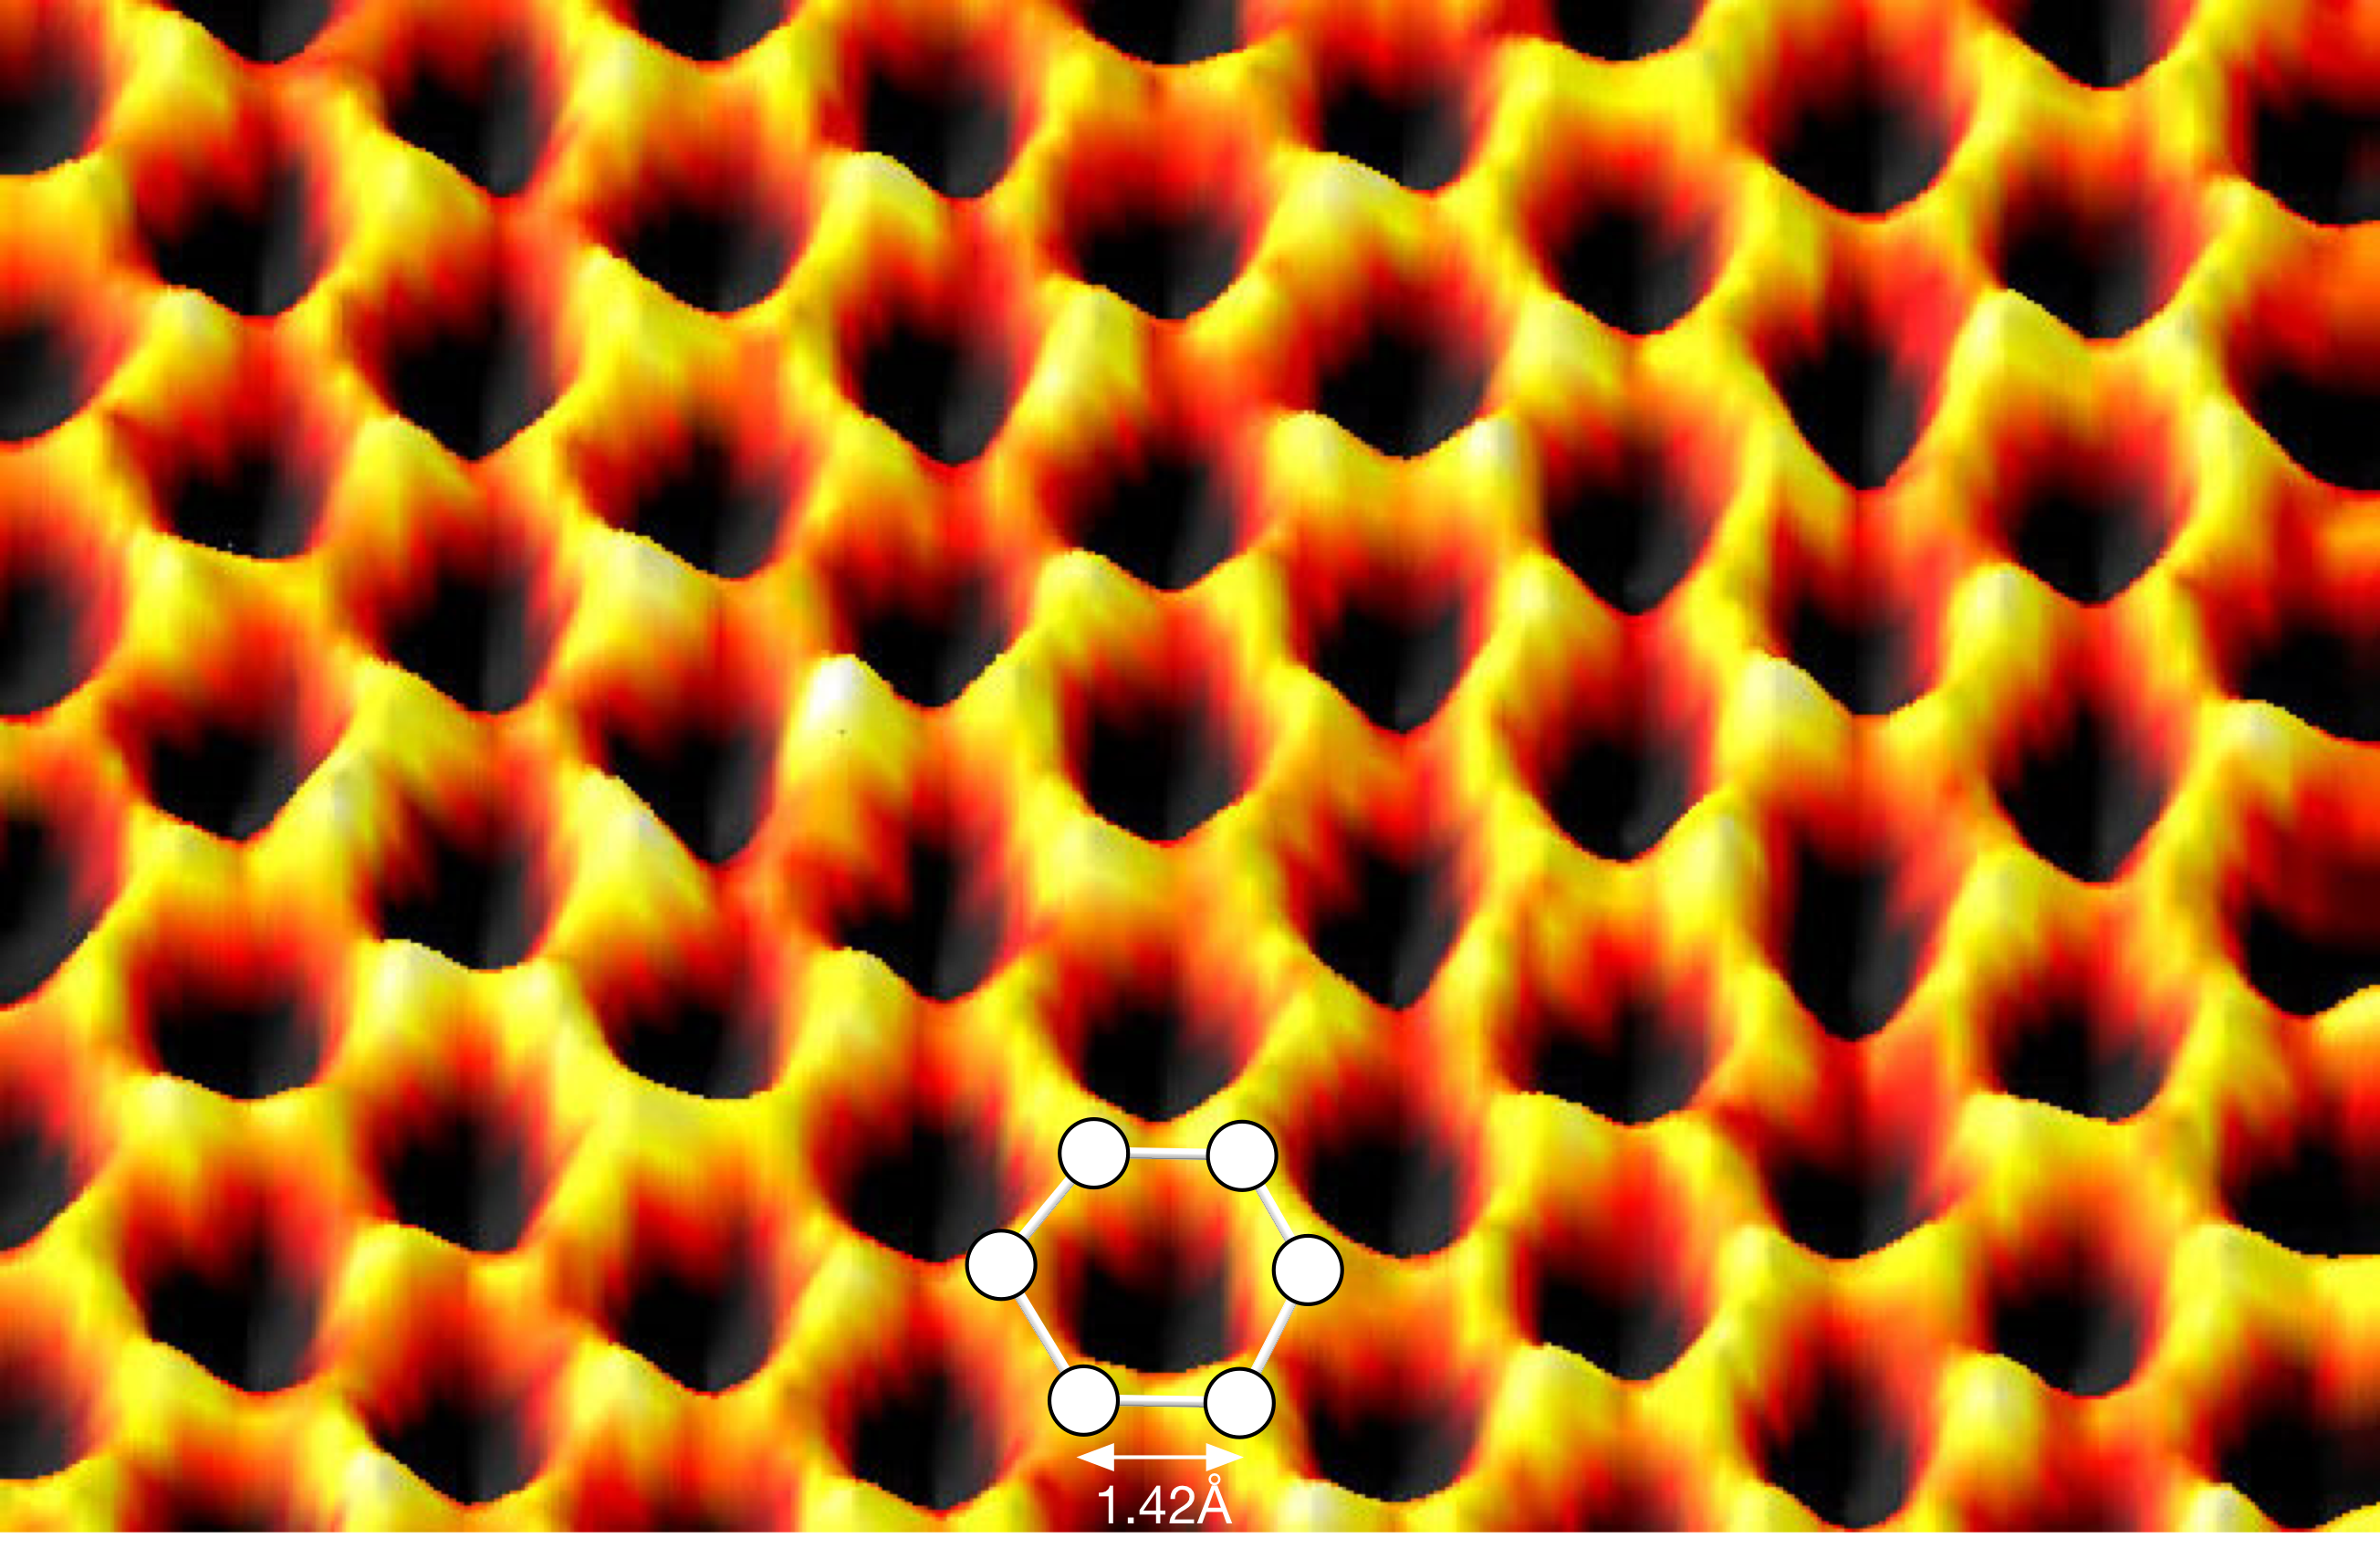
\includegraphics[width=0.7\textwidth]{./images/graphene-spm.png}
  \caption{Graphene's two dimensional hexagonal structure as seen through scanning tunnerling microscopy. The distance between two atoms is about \SI{1.42}{\angstrom} (adapted from \cite{graphene-spm}). One hexagon is exemplarily highlighted.}
  \label{fig:spm}
\end{figure}

As seen in figure~\ref{fig:lattice}a graphene's lattice consists of a two-atom triangular Bravais lattice which is spanned by the two basis vectors $\mathbf{a}_1$ and $\mathbf{a}_2$. For solid state physics it is often interesting to look at the corresponding lattice in $k$-space. Graphene's reciprocal lattice is also hexagonal with a hexagonal unit cell with $\Gamma$ as its center (as seen in figure~\ref{fig:lattice}b). Other symmetric points are $K_+$ and $K_-$ at the corners of the first Brillouin zone. In addition to them there is the $M$ point describing the center between $K_+$ and $K_-$.

\begin{figure}[!h]
  \centering
  \begin{subfigure}{0.45\textwidth}
    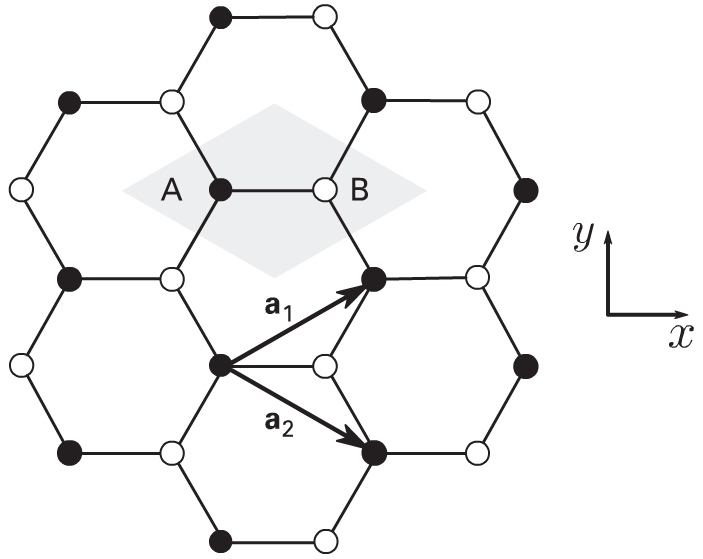
\includegraphics[width=\textwidth]{./images/cell.png}
  \end{subfigure}
  ~
  \begin{subfigure}{0.45\textwidth}
    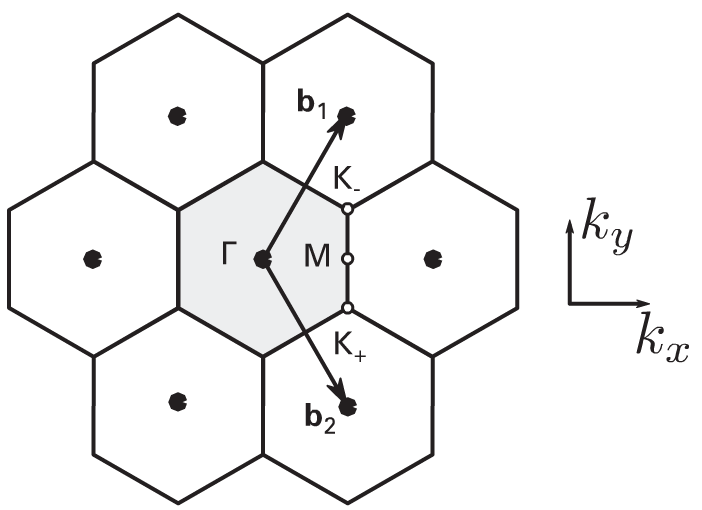
\includegraphics[width=\textwidth]{./images/k-cell.png}
  \end{subfigure}
  \caption{\textbf{(a)} The basis vectors $\mathbf{a}_1$ and $\mathbf{a}_2$ build a triangular Bravais lattice with a two atom basis. The Wigner-Seitz cell is shaded in gray (adapted from \mcite). \textbf{(b)} The reciprocal lattice with the unit cell shaded in gray. $\Gamma$ is the cell's center; $K_+$, $K_-$ and $M$ are high-symmetry points (adapted from \mcite). \note{add labels}}
  \label{fig:lattice}
\end{figure}

\newpage

\subsubsection{Electronic Properties}

Most of graphene's special electronic properties are caused by the fourth valence electron which causes the $\pi$ orbitals to hybridize and form a delocalized electron cloud above and below the graphene lattice enabling ballistic transport of electrons and a high carrier mobility\cite{carrier}. These orbitals are depicted in figure~\ref{fig:orbitals}.

\begin{figure}[!h]
  \centering
  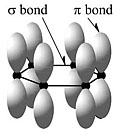
\includegraphics[width=0.3\textwidth]{./images/orbitals.jpg}
  \caption{Valence orbitals of carbon atoms in graphene. Covalent bonds are formed from $\sigma$-orbitals while the perpendicular $\pi$-orbitals create the valence and conduction band. Adapted from http://www.andrew.cmu.edu/user/feenstra/graphene/\mcite. \note{redraw pixeled labels}}
  \label{fig:orbitals}
\end{figure}

Due to the symmetry of the system the $\pi$ orbitals can be treated independently as the main contributor to the conduction and valence band. The band structure can be calculated with a tight-binding model as\cite{dispersion}

\begin{equation}
  E(\mathbf{k})=\pm\sqrt{\gamma_0^2\left(1+4\cos^2\frac{k_ya}{2}+4\cos\frac{k_ya}{2}\cdot\cos\frac{k_x\sqrt{3}a}{2}\right)},
  \label{eq:dispersion}
\end{equation}

with the hopping energy $\gamma_0\approx\SI{2.8}{eV}$\cite{dispersion}, the lattice constant $a\approx\SI{2.46}{Å}$, "$+$" for the conduction band and "$-$" for the valence band.

A plot of the band structure in figure~\ref{fig:bands} shows that valence and conduction band touch in the $K$-points. Looking a bit closer at the band structure near the $K$ points in figure~\ref{fig:bands} allows to use a linear approximation of the valence and conduction band. Both bands touch in a single point at the intersection.

\begin{figure}[!h]
  \centering
  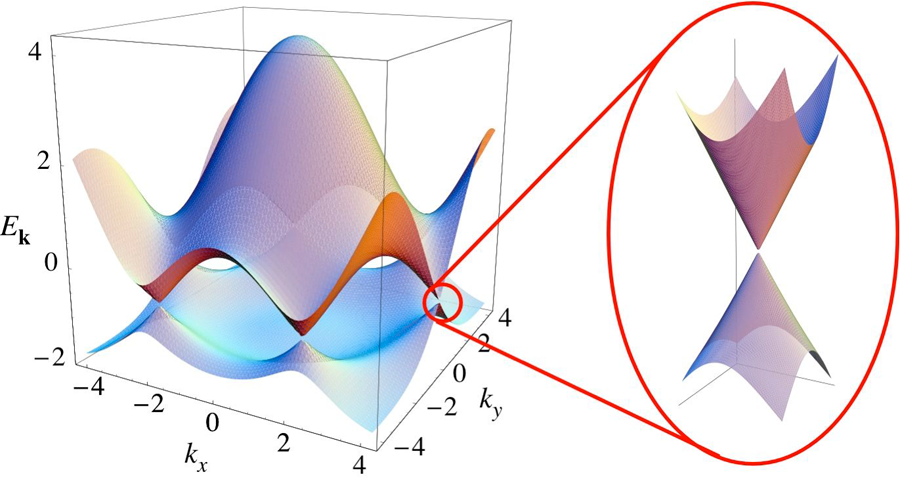
\includegraphics[width=0.8\textwidth]{./images/dispersion.png}
  \caption { Conduction and valence band touch in the points $K_-$ and $K_+$. At these points the conduction and valence bands can be linearly approximated (figure from \cite{graphene}). }
  \label{fig:bands}
\end{figure}

Evaluating equation~(\ref{eq:dispersion}) at the K points gives

\begin{equation}
  E(\mathbf{K})=0,
\end{equation}

confirming that conduction and valence band touch in the K points and therefore graphene is a semiconductor without a band gap.

\subsubsection{Other Properties}

Other interesting properties of graphene often exceed those of any other material. It has an intrinsic tensile strength of 130 GPa and a Young's modulus as high as 1TPa\cite{strength}. It is also impermeable to gases\cite{Bunch2008} and absorbs light by a factor of $\pi\alpha$\cite{optical}, where $\alpha$ is the fine structure constant.
